\documentclass[a4paper,11pt]{article}
%\documentclass[a4paper,11pt,fleqn]{article}

\setlength{\textwidth}{160mm} 
\setlength{\oddsidemargin}{0mm} 
\setlength{\evensidemargin}{0mm} 
\setlength{\topmargin}{-2.2mm} % = 0mm -1in + 23.2mm 
\setlength{\textheight}{221.9mm} % = 297mm -29.5mm -31.6mm - 14mm (12 to accomodate footline with pagenumber)
\setlength{\headheight}{14pt}
%%%%%%%%%%%%%%%%%%%%%%%%%%%%%%%%%%%%%%%%%%%%%%

\usepackage{graphicx}
\usepackage{xcolor}

\usepackage{amsmath}
\usepackage{amssymb}

\setcounter{topnumber}{2}
\setcounter{bottomnumber}{2}
\setcounter{totalnumber}{4}     % 2 may work better
%\setcounter{dbltopnumber}{2}    % for 2-column pages
\author{Gr\'egoire A. Gallet and Fabio Pietrucci}
\title{\texttt{piv\_clustering} v1.3\\ {\color{blue}structural clustering of atomic trajectories \\ based on the Permutation Invariant Vector}}

%%%%%%%%%%%%%%%%%%%%%%%%%%%%%%%%%%%%%%%%%%%%%%%%%%%%%%%%%%%%%%%%%%%%%%
\begin{document}
\maketitle
This short manual presents the basic functionalities of the \texttt{piv\_clustering} utility;
the theory and two applications are detailed in
\begin{center} {\large G. A. Gallet and F. Pietrucci; J. Chem. Phys. \textbf{139}, 074101 (2013) \\
doi: \texttt{10.1063/1.4818005}}\end{center}
If you are using the code, please read and cite this paper.\\
\begin{figure}[!ht]
  \centering
  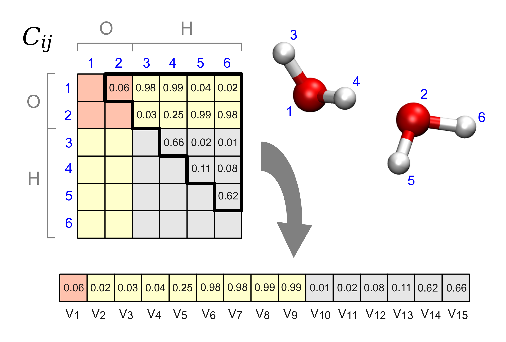
\includegraphics[width=0.6\textwidth]{./piv.eps}
\end{figure}

The \texttt{piv\_clustering} utility is available free of charge at 
\begin{center}
\texttt{http://sourceforge.net/projects/pivclustering/} \\ 
\end{center}
You can redistribute it and/or modify it under the
terms of the GNU General Public License as published by the Free
Software Foundation, either version 3 of the License, or (at your option)
any later version. Our code is distributed in the hope that it will be useful,
but WITHOUT ANY WARRANTY; without even the implied warranty of
MERCHANTABILITY or FITNESS FOR A PARTICULAR PURPOSE. See
the GNU General Public License for more detail. You should have
received a copy of the GNU General Public License along with our code.
If not, see \texttt{http://www.gnu.org/licenses/}.\\

\newpage

%%%%%%%%%%%%%%%%%%%%%%%%%%%%%%%%%%%%%%%%%%%%%%%%%%%%%%%%%%%%%%%%%%%%%%
\section{Compilation}
  Compiling should be straightforward  with \texttt{gfortran} and \texttt{openmpi}:
  just \texttt{make} in the directory where you decompressed piv\_clustering\_1.3.tar.gz.
  In case you want to compile a serial version (not parallel), modify the file \texttt{makefile} by removing the flag
  \texttt{-DMPI} and replacing \texttt{mpif90} with \texttt{gfortran}.
  Other compiling schemes have not been tested extensively.

%%%%%%%%%%%%%%%%%%%%%%%%%%%%%%%%%%%%%%%%%%%%%%%%%%%%%%%%%%%%%%%%%%%%%%
\section{Input}
  The clustering program currently analyzes trajectories written in the formats xyz and pdb.
  In the case of xyz files, only orthorombic simulation boxes are supported, with fixed $a\ b\ c$ sides.
  In the case of pdb files, triclinic cells are allowed, and the parameters $a\ b\ c\ \alpha\ \beta\ \gamma$ 
  are specified for each frame, so that variable cells can be employed
  (note that there was a bug in version 1.2, fixed in version 1.3). 
  All details about file formats 
  are discussed in Section 3. Starting from the atomic coordinates, a Permutation Invariant Vector (PIV)
  is constructed for each trajectory frame, and the matrix of distances between all pairs of PIVs is computed.
  Frames are then clusterized into disjoint sets employing different algorithms.

  Executing \texttt{./piv\_clustering.x} will print the following tips:
\begingroup\fontsize{8pt}{12pt}\selectfont
\begin{verbatim}
====================================================
===        P I V      C L U S T E R I N G        ===
====================================================
 version 1.3 - G. A. Gallet and F. Pietrucci, 2014  
 please read and cite J.Chem.Phys.139,074101(2013)  
            < running on   1 procs >
 
USAGE:
./piv_clustering.x -filexyz traj.xyz -bsize 12.1 8.2 10.4 -method 2 -coord1_range 1.0 4.0 -algorithm 50 ...

[-filepdb          ] input trajectory file (pdb format, includes cell parameters)
[-filexyz          ] input trajectory file (xyz format)
[-bsize            ] orthorombic box sides a b c in angstrom (only for xyz format)
[-out              ] prefix for output cluster files (default cluster?.xyz)
[-array_size       ] size of the biggest array allocated by the program
[-method           ] method used to compute the PIV 1: distance, 2: coordination, 3: sprint
[-coord1_range     ] specify the two distances at which coordination = 0.9 and 0.1, respectively
[-coord1_param     ] parameters d0 r0 of coordination function 1/(1+exp((d-d0)/r0)) (method 2 or 3)
[-coord2_param     ] parameters d0 r0 m n of coordination function (1-x**m)/(1-x**n) with x=(d-d0)/r0 (method 2 or 3)
[-nosort           ] specify if you do not want to enforce the permutation symmetry of identical atoms
[-restart_piv      ] restart the PIV from PIV_CORE.?  (it requires the same number of cores!)
[-restart_matrix   ] restart the matrix from FRAME_TO_FRAME.MATRIX (also skip the PIV computation)
[-algorithm        ] clustering algorithm 1: Daura's, >1: kmedoids with the number indicating the number of clusters
[-cutoff_daura     ] cutoff for Daura's algorithm
[-cutoff_clcoeff   ] cutoff for computing the clustering coefficient
[-network_analysis ] analyze the network formed by cluster centers, and plot it in network.svg
[-rdf              ] writes the radial distribution function g(r) in file rdf.dat              
\end{verbatim}
\endgroup

\newpage

  \begin{description}
  \item[\texttt{-filepdb}           ]\hfill\\
                                       {\color{red}required} (or alternatively \texttt{-filexyz}). The trajectory file in pdb format 
                                       (see Section 3 for details). 
  \item[\texttt{-filexyz}           ]\hfill\\
                                       {\color{red}required} (or alternatively \texttt{-filepdb}). The trajectory file in xyz format 
                                       (see Section 3 for details).
  \item[\texttt{-bsize}             ]\hfill\\
                                       {\color{red}required} (only with \texttt{-filexyz}). The box sides $a\ b\ c$ in angstrom units 
                                       (currently only orthorombic cells are allowed) for the xyz trajectory file.
  \item[\texttt{-out}               ]\hfill\\
                                       {\color{green}optional}. You can provide a prefix for the output cluster files.
  \item[\texttt{-array\_size}       ]\hfill\\
                                       {\color{green}optional}. It limits the size of the biggest arrays (\texttt{reduced\_piv}
                                       in the code); default is $10^8$ elements (each element is \texttt{double\_precision}). If
                                       the code crashes at runtime because of a lack of memory, try to reduce this number.
  \item[\texttt{-method}            ]\hfill\\
                                       {\color{red}required}. Method employed to compute the components of the PIV: 1) 
                                       plain interatomic Cartesian distance, 2) coordination function (see below), 3) SPRINT \cite{sprint}.
                                       If methods 2 or 3 are chosen, the user must specify the coordination function to be used, 
                                       using one and only one of the keywords \texttt{-coord1\_param}, \texttt{-coord1\_range}, \texttt{-coord2\_param}.
  \item[\texttt{-coord1\_param}     ]\hfill\\
                                       {\color{red}required} (only for \texttt{-method 2} or \texttt{3}, inactive for \texttt{-method 1}). 
                                       The parameters $d_0$, $r_0$ of the coordination function 
                                       \begin{equation*}
                                         C(d)=\frac{1}{1+\exp((d-d_0)/r_0)}
                                       \end{equation*}
                                       must be provided, where $d$ is the interatomic Cartesian distance. 
                                       Note that \texttt{-coord1\_param} and \texttt{-coord1\_range} are mutually exclusive.
  \item[\texttt{-coord1\_range}     ]\hfill\\
                                       {\color{red}required} (only for \texttt{-method 2} or \texttt{3}, inactive for \texttt{-method 1}). 
                                       The two interatomic distances at which the coordination function above assumes the values 0.9 and 0.1 
                                       must be provided. 
                                       The parameters $d_0$ and $r_0$ are calculated automatically. 
                                       Note that \texttt{-coord1\_param} and \texttt{-coord1\_range} are mutually exclusive.
  \item[\texttt{-coord2\_param}     ]\hfill\\
                                       {\color{red}required} (only for \texttt{-method 2} or \texttt{3}, inactive for \texttt{-method 1}). 
                                       The parameters $d_0$, $r_0$, $m$ and $n$ for
                                       the coordination function 
                                       \begin{equation*}
                                         C(d)=\frac{1-\left(\frac{d-d_0}{r_0}\right)^m}{1-\left(\frac{d-d_0}{r_0}\right)^n}
                                       \end{equation*}
                                       must be provided, where $d$ is the interatomic Cartesian distance. 
  \item[\texttt{-nosort}            ] \hfill\\
                                       {\color{green}optional}. You should specify this only if you do not want to 
                                       sort the PIV, i.e.,  you do not want the magic of our method at work.
  \item[\texttt{-restart\_piv} ]\hfill\\
                                       {\color{green}optional}. Reads back the PIV from \texttt{PIV\_CORE.*}
                                       files rather than computing them. You need to have the same number of cores
                                       reading them than when you first wrote them. This option is meaningless 
                                       if \texttt{restart\_matrix} is specified.
  \item[\texttt{-restart\_matrix}   ]\hfill\\
                                       {\color{green}optional}. 
                                       Reads back the frame to frame
                                       distance matrix from the file \texttt{FRAME\_TO\_FRAME.MATRIX} rather than
                                       computing it from the PIV. This option is very useful since computing
                                       this matrix is the most expensive part of the calculation.
  \item[\texttt{-algorithm}         ]\hfill\\
                                       {\color{red}required}. Can be either 1 or $>1$: in the former case, Daura's algorithm
                                       \cite{daura} is employed to cluster the data. In the latter, kmedoids \cite{kmedoids}
                                       with k-means++ initialization \cite{kmeans} is employed and the number
                                       is the desired number of clusters.
  \item[\texttt{-cutoff\_daura}     ]\hfill\\
                                       {\color{red}required} (only for \texttt{-algorithm 1}). Specifies the cutoff (in PIV units) for Daura's 
                                       clustering algorithm \cite{daura}. To have a clue about reasonable values, check the average and maximum
                                       distance between frames as printed in the output of the program.
  \item[\texttt{-cutoff\_clcoeff}   ]\hfill\\
                                       {\color{green}optional}. Specifies a cutoff (in PIV units) to define when two members of a cluster are
                                       neighbor. Used only for computing the clustering coefficient.
  \item[\texttt{-network\_analysis} ]\hfill\\
                                       {\color{green}optional}. Generates a map of the cluster centers in \texttt{svg} format.
  \item[\texttt{-rdf}               ]\hfill\\
                                       {\color{green}optional}. Writes the radial distribution function g(r) and the number of atoms
                                        within a radius r N(r) in file \texttt{rdf.dat}.
  \end{description}

\newpage

%%%%%%%%%%%%%%%%%%%%%%%%%%%%%%%%%%%%%%%%%%%%%%%%%%%%%%%%%%%%%%%%%%%%%%
\section{Trajectory file formats}

As a general remark, the program identifies identical atoms as those that have the same symbol in the trajectory file. 
Identical atoms are considered indistinguishable, thus thay can be exchanged without changing the physical properties of the system.
Therefore, if for some reason you want to keep two atoms of the same element as distinguishable, label them with different symbols in the 
trajectory file, e.g., C1 and C2 instead of C and C.

BEWARE: each frame in the trajectory file must have the same sequence of chemical elements, otherwise the program will print
incorrect results. 
In other words, a configuration with sequence "O O O H H H H H H" cannot be compared with "O H H O H H O H H"; chemical elements 
must match in all frames.

\subsection{pdb format}

Example:
\begingroup\fontsize{8pt}{12pt}\selectfont
\begin{verbatim}
CRYST1   20.245   22.023   20.327  90.55  86.06  90.04 P 1           1
MODEL       1    amorphous ice
ATOM      1  O   SOL     1       3.870   1.172  20.453  1.00  0.00            
ATOM      2  H   SOL     1       3.840   1.190  19.497  1.00  0.00            
ATOM      3  H   SOL     1       4.621   1.719  20.681  1.00  0.00            
ATOM      4  O   SOL     2       3.630  21.799   3.621  1.00  0.00            
ATOM      5  H   SOL     2       2.858  21.248   3.753  1.00  0.00            
ATOM      6  H   SOL     2       4.201  21.280   3.055  1.00  0.00
  ...
CRYST1   20.246   22.128   20.345  90.16  86.34  90.33 P 1           1
MODEL       2    amorphous ice
ATOM      1  O   SOL     1       2.579   1.200   0.349  1.00  0.00
ATOM      2  H   SOL     1       2.393   1.110  -0.586  1.00  0.00
ATOM      3  H   SOL     1       3.374   1.733   0.384  1.00  0.00
ATOM      4  O   SOL     2       3.709  21.884   3.893  1.00  0.00
ATOM      5  H   SOL     2       3.030  21.235   4.080  1.00  0.00
ATOM      6  H   SOL     2       4.298  21.445   3.279  1.00  0.00
  ...
\end{verbatim}
\endgroup
Each frame must contain the records \texttt{CRYST1 MODEL ATOM}; additional records are ignored.
According to the official pdb format (\texttt{http://www.wwpdb.org/docs.html}) the record \texttt{CRYST1}
contains at columns 7-54 the $a\ b\ c\ \alpha\ \beta\ \gamma$ cell parameters,
where $\alpha$ is the angle (in degrees) between vectors \textbf{b} and \textbf{c},
$\beta$ between \textbf{a} and \textbf{c}, and $\gamma$ between \textbf{a} and \textbf{b}.
The record \texttt{MODEL} contains a comment.
The record \texttt{ATOM} contains the atom symbol at columns 13-16, and the Cartesian coordinates at columns 31-54; additional 
information on the same line is ignored.

\subsection{xyz format}

Example:
\begingroup\fontsize{8pt}{12pt}\selectfont
\begin{verbatim}
1080
 step  1    amorphous ice
O     3.870   1.172  20.453 
H     3.840   1.190  19.497 
H     4.621   1.719  20.681 
O     3.630  21.799   3.621 
H     2.858  21.248   3.753 
H     4.201  21.280   3.055 
  ...
1080
 step  2    amorphous ice
O     2.579   1.200   0.349  
H     2.393   1.110  -0.586  
H     3.374   1.733   0.384  
O     3.709  21.884   3.893  
H     3.030  21.235   4.080  
H     4.298  21.445   3.279  
  ...
\end{verbatim}
\endgroup
Each frame begins with a line containing the number of atoms, followed by a comment line, followed by a line per atom
containing the atom symbol and the Cartesian coordinates. Contrary to the pdb format, there are no predefined column ranges.
The cell parameters are fixed and provided as a command line input with \texttt{-bsize}.

%%%%%%%%%%%%%%%%%%%%%%%%%%%%%%%%%%%%%%%%%%%%%%%%%%%%%%%%%%%%%%%%%%%%%%

\section{Output}
  \texttt{piv\_clustering} generates several output files:
  \begin{description}
  \item[\texttt{PIV\_CORE.*}]\hfill\\
                                                            Temporary binary files used to store the PIV of each
                                                            frame. One file is written for each CPU. They can be used to
                                                            restart a calculation (keyword \texttt{-restart\_piv}).
                                                            They are not required if the calculation is restarted from
                                                            \texttt{FRAME\_TO\_FRAME.MATRIX} (keyword \texttt{-restart\_matrix}).
  \item[\texttt{FRAME\_TO\_FRAME.MATRIX}         ]\hfill\\
                                                            Human-readable file containing the complete frame to frame distance matrix. 
                                                            It is heavy to compute and you should restart from it 
                                                            (keyword \texttt{-restart\_matrix}) 
                                                            if you do not modify the definition of the PIV components. 
                                                            The first line contains the dimension of the square matrix (i.e., the number of 
                                                            trajectory frames) and the maximum distance between frames.
                                                            The next lines contain the matrix elements (scaled by the maximum distance).
  \item[\texttt{centers.xyz}                     ]\hfill\\
                                                            An xyz file including all the cluster centers. The comment lines 
                                                            contain relevant information you might want to look at.
  \item[\texttt{cluster*.xyz}                    ]\hfill\\
                                                            One xyz file per cluster, containing all the cluster members. 
                                                            For each member, its distance from the center is printed in the comment line.
  \item[\texttt{network.svg}                     ]\hfill\\
                                                            A svg file (which you can see, e.g.,  with Inkscape or Firefox) sketching
                                                            the network of cluster centers (keyword \texttt{-network\_analysis}).
  \end{description}

                        
%%%%%%%%%%%%%%%%%%%%%%%%%%%%%%%%%%%%%%%%%%%%%%%%%%%%%%%%%%%%%%%%%%%%%%
\newpage                        
\section{Example}
  Here below is a simple example for testing purposes, in directory \texttt{test}. 

  The trajectory \texttt{traj-ice-melting.xyz} is taken from a simulation of ice at 320K
  (64 water molecules, TIP4P potential). The ice starts melting at around step 70.
  If you did not compile the mpi version of the code, remove "mpirun -np 4" from the commands below.
  First, try to execute the commands in file \texttt{run1} (Daura's clustering algorithm):
  \begin{verbatim}
mpirun -np 4 ../piv_clustering.x -filexyz traj-ice-melting.xyz -bsize 12.8 12.8 12.8 \ 
-method 2 -coord1_param 2.6 0.6 -algorithm 1 -cutoff_daura 1.2 &> log1
  \end{verbatim}
  Two clusters will be found, and you should obtain a similar output as in directory \texttt{test/check1}. 
  The calculation should require a few seconds.

  Afterwards, you can restart the distance matrix in file \texttt{FRAME\_TO\_FRAME.MATRIX} (very quick, especially in the case of large trajectories) 
  and try instead the k-medoids algorithm with 2 clusters:
  \begin{verbatim}
mpirun -np 4 ../piv_clustering.x -filexyz traj-ice-melting.xyz -bsize 12.8 12.8 12.8 \
-method 2 -coord1_param 2.6 0.6 -algorithm 2 -restart_matrix &> log2
  \end{verbatim}
  Note: keep in mind that the k-means++ initialization of the k-medoids algorithm is based on random numbers, 
  therefore the clustering results may differ repeating the same command: test several times to 
  ensure that results are robust.
  In particular, your result may differ from those in directory \texttt{test/check2}.
  Daura's algorithm instead is reproducible, but does not allow to specify in advance the desired number of clusters.
\begin{figure}[!ht]
  \centering
  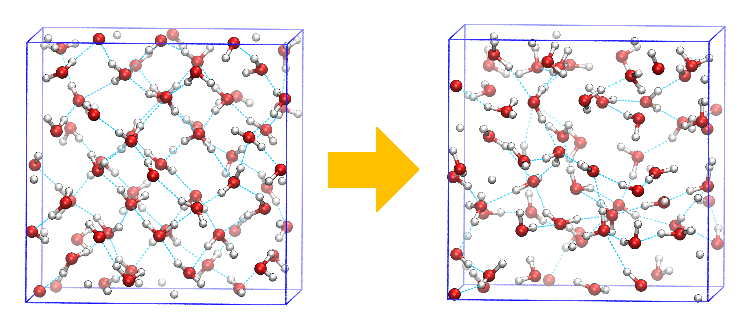
\includegraphics[width=12cm]{./ice-melting.eps}
\end{figure}

%%%%%%%%%%%%%%%%%%%%%%%%%%%%%%%%%%%%%%%%%%%%%%%%%%%%%%%%%%%%%%%%%%%%%%
\newpage
\bibliographystyle{unsrt}% not to be used with numbers
\bibliography{bibliography}

\end{document}
